%\chapter{Supercondensadores}
\noindent
\rule{\linewidth}{1 pt}
\begin{flushright}
	\begin{quotation}
		\small{
			\textit{``The force is strong with this one.''}}
	\end{quotation}
	\bf{Darth Vader}
\end{flushright}
\noindent
\rule{\linewidth}{1 pt}\\
\vfill

%ENERGY STORAGE
El almacenar energía eléctrica es uno de los mayores problemas a la hora de diseñar sistemas electrónicos tanto móviles como estacionarios, los requerimientos varían de acuerdo a las necesidades de cada uno, en general es un \textit{trade-off} entre densidad de energía (cuánta energía se puede almacenar) y densidad de potencia (que tan rápido puede ser entregada la energía almacenada). Las celdas de combustible (\textit{Fuel Cells}), entregan la mayor densidad de energía, pero son complicadas, mientras que las baterías poseen mayor densidad de potencia, pierden capacidad con los ciclos de carga y descarga. Los supercondensadores van un paso más allá, aumentado la densidad de potencia y aportando mayor vida útil, entregando una nueva posibilidad a la hora de diseñar sistemas eléctricos, ya como fuente de energía por sí mismo, o en sistemas híbridos combinados con otras tecnologías\cite{Thounthong2009}.
\section{El condensador ideal\index{condensador ideal}}
Generalmente un condensador se modela como un par de placas paralelas separadas por un dieléctrico, es definido por su capacitancia, la que refleja la capacidad de almacenar energía. Del modelo de placas paralelas se desprende la definición de capacitancia $C$ como la razón entre la magnitud de carga en cada placa $Q$ y el voltaje entre los terminales $V$:

\begin{equation}
	C = \frac{Q}{V}
\end{equation}

Para fines prácticos, el condensador ideal como componente electrónico es modelado por la ecuación que relaciona la corriente con el voltaje, considerando que $i = dq/dt$:

\begin{equation}
	i(t) = C \frac{dv(t)}{dt}
\end{equation}

Para corrientes constantes, el voltaje varía linealmente como en la carga y descarga de la figura \ref{fig:plot:charge-discharge_ideal_cap}.
\begin{figure}[h!]
	\fbox{
		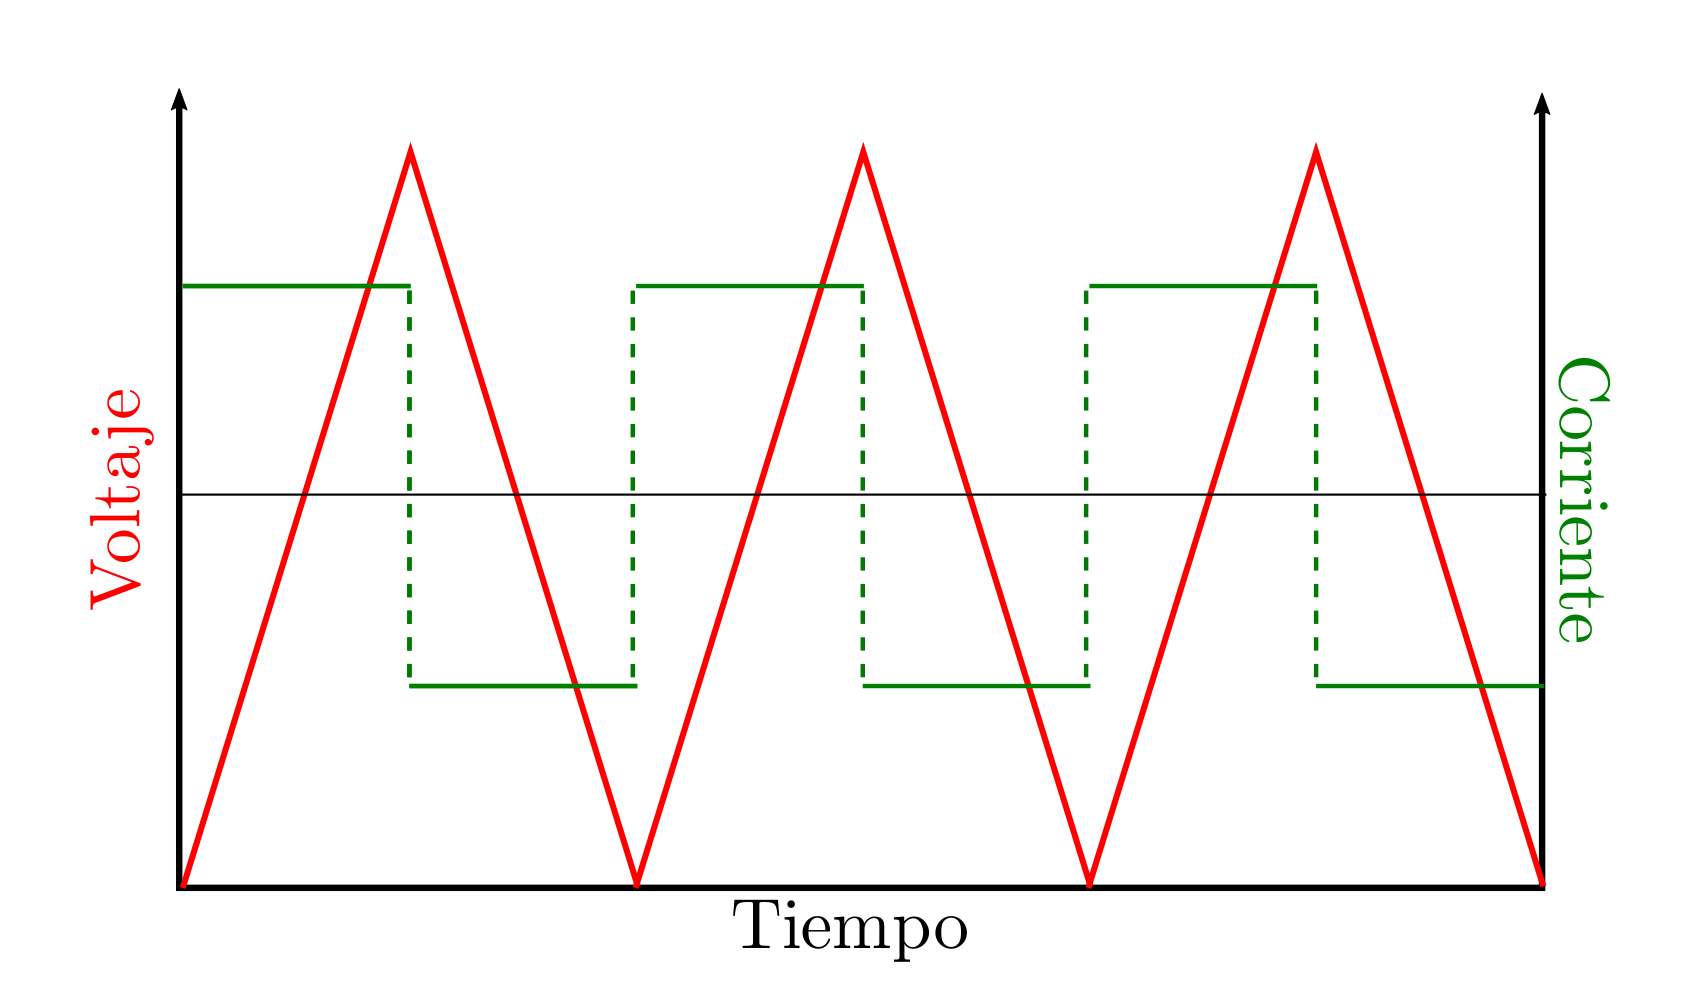
\includegraphics[width=\textwidth]{charge-discharge_ideal_cap.png}
		}
	\caption{Carga y descarga de un condensador ideal a corriente constante.}
	\label{fig:plot:charge-discharge_ideal_cap}
\end{figure}

\section{El condensador real\index{condensador real}}
Un condensador ideal almacenaría energía al cargase y la entregaría al descargarse sin ninguna disipación, es decir, su eficiencia sería del 100\%, podría soportar cualquier voltaje aplicado o cargarse y descargarse por una corriente cuan grande se desee.  En realidad, los condensadores sí disipan energía, poseen voltajes de operación y corrientes máximas de carga y descarga. Todo esto depende de como fue construido y qué materiales se utilizaron, pensando en su propósito.

\subsection{Breakdown voltage}
Los condensadores convencionales construidos con materiales dieléctricos están sujetos a un voltaje máximo de operación determinado por la tensión de ruptura (\textit{Breakdown voltage})\index{tensión de ruptura, \textit{breakdown voltage}}, voltaje al cual se pierden las propiedades dieléctricas del material ocasionando cortocircuito al interior del dispositivo, determinado por la fuerza dieléctrica del material y el espesor de este. En los condensadores electrolíticos la tensión de ruptura es determinada por otros mecanismos\cite{Yahalom1971}. En lo que respecta a los supercondensadores, el voltaje máximo de carga depende fundamentalmente de electrolíto usado, principalmente por las reacciones que ocurren a ciertos potenciales, este tema será abordado con más detalle en la sección correspondiente.

\subsection{Circuito equivalente}
El comportamiento de los condensadores reales son modeladas por un circuito equivalente, donde se introducen componentes que representan las imperfecciones del funcionamiento del condensador real.\\

\subsection{Resistencia en serie equivalente (ESR)}
Las imperfecciones en la construcción de los electrodos, y la naturaleza de los materiales utilizados (e.g. resistencia no cero), disipan energía durante la carga y descarga como si se tratase de una resistencia en serie al condensador, esto se ve reflejado como una caída de voltaje en los terminales del dispositivo (figura \ref{fig:plot:charge-discharge_esr}), y disminuye la eficiencia de éste.

\begin{figure}[h!]
	\fbox{
		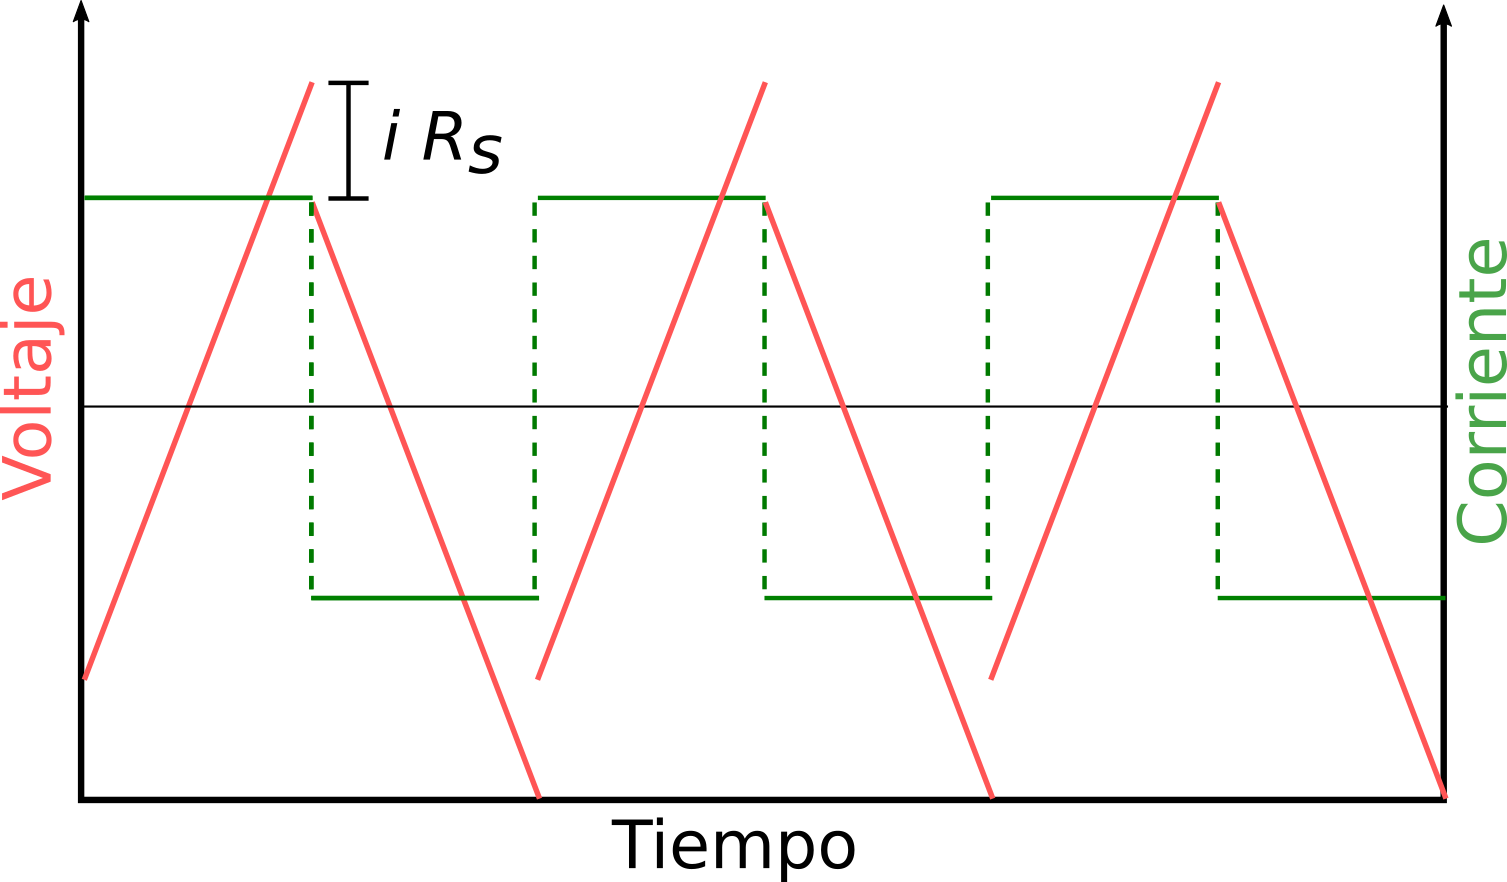
\includegraphics[width=\textwidth]{charge-discharge_esr.png}
	}
	\caption{Carga y descarga de un condensador evidenciando el efecto de una ESR.}
	\label{fig:plot:charge-discharge_esr}
\end{figure}

\subsection{Corriente de fuga (\emph{leakage current})}
Entre los electrodos del condensador fluye una corriente no deseada cuando existe una diferencia de potencial entre los electrodos, esta corriente 

\section{¿Qué hace a un supercondensador super?}

\subsection{Doble capa electrostática de Helmholtz}
La gran densidad de energía de un supercondensador respecto a uno convencional

\begin{figure}[h!]
	\centering
	\fbox{
		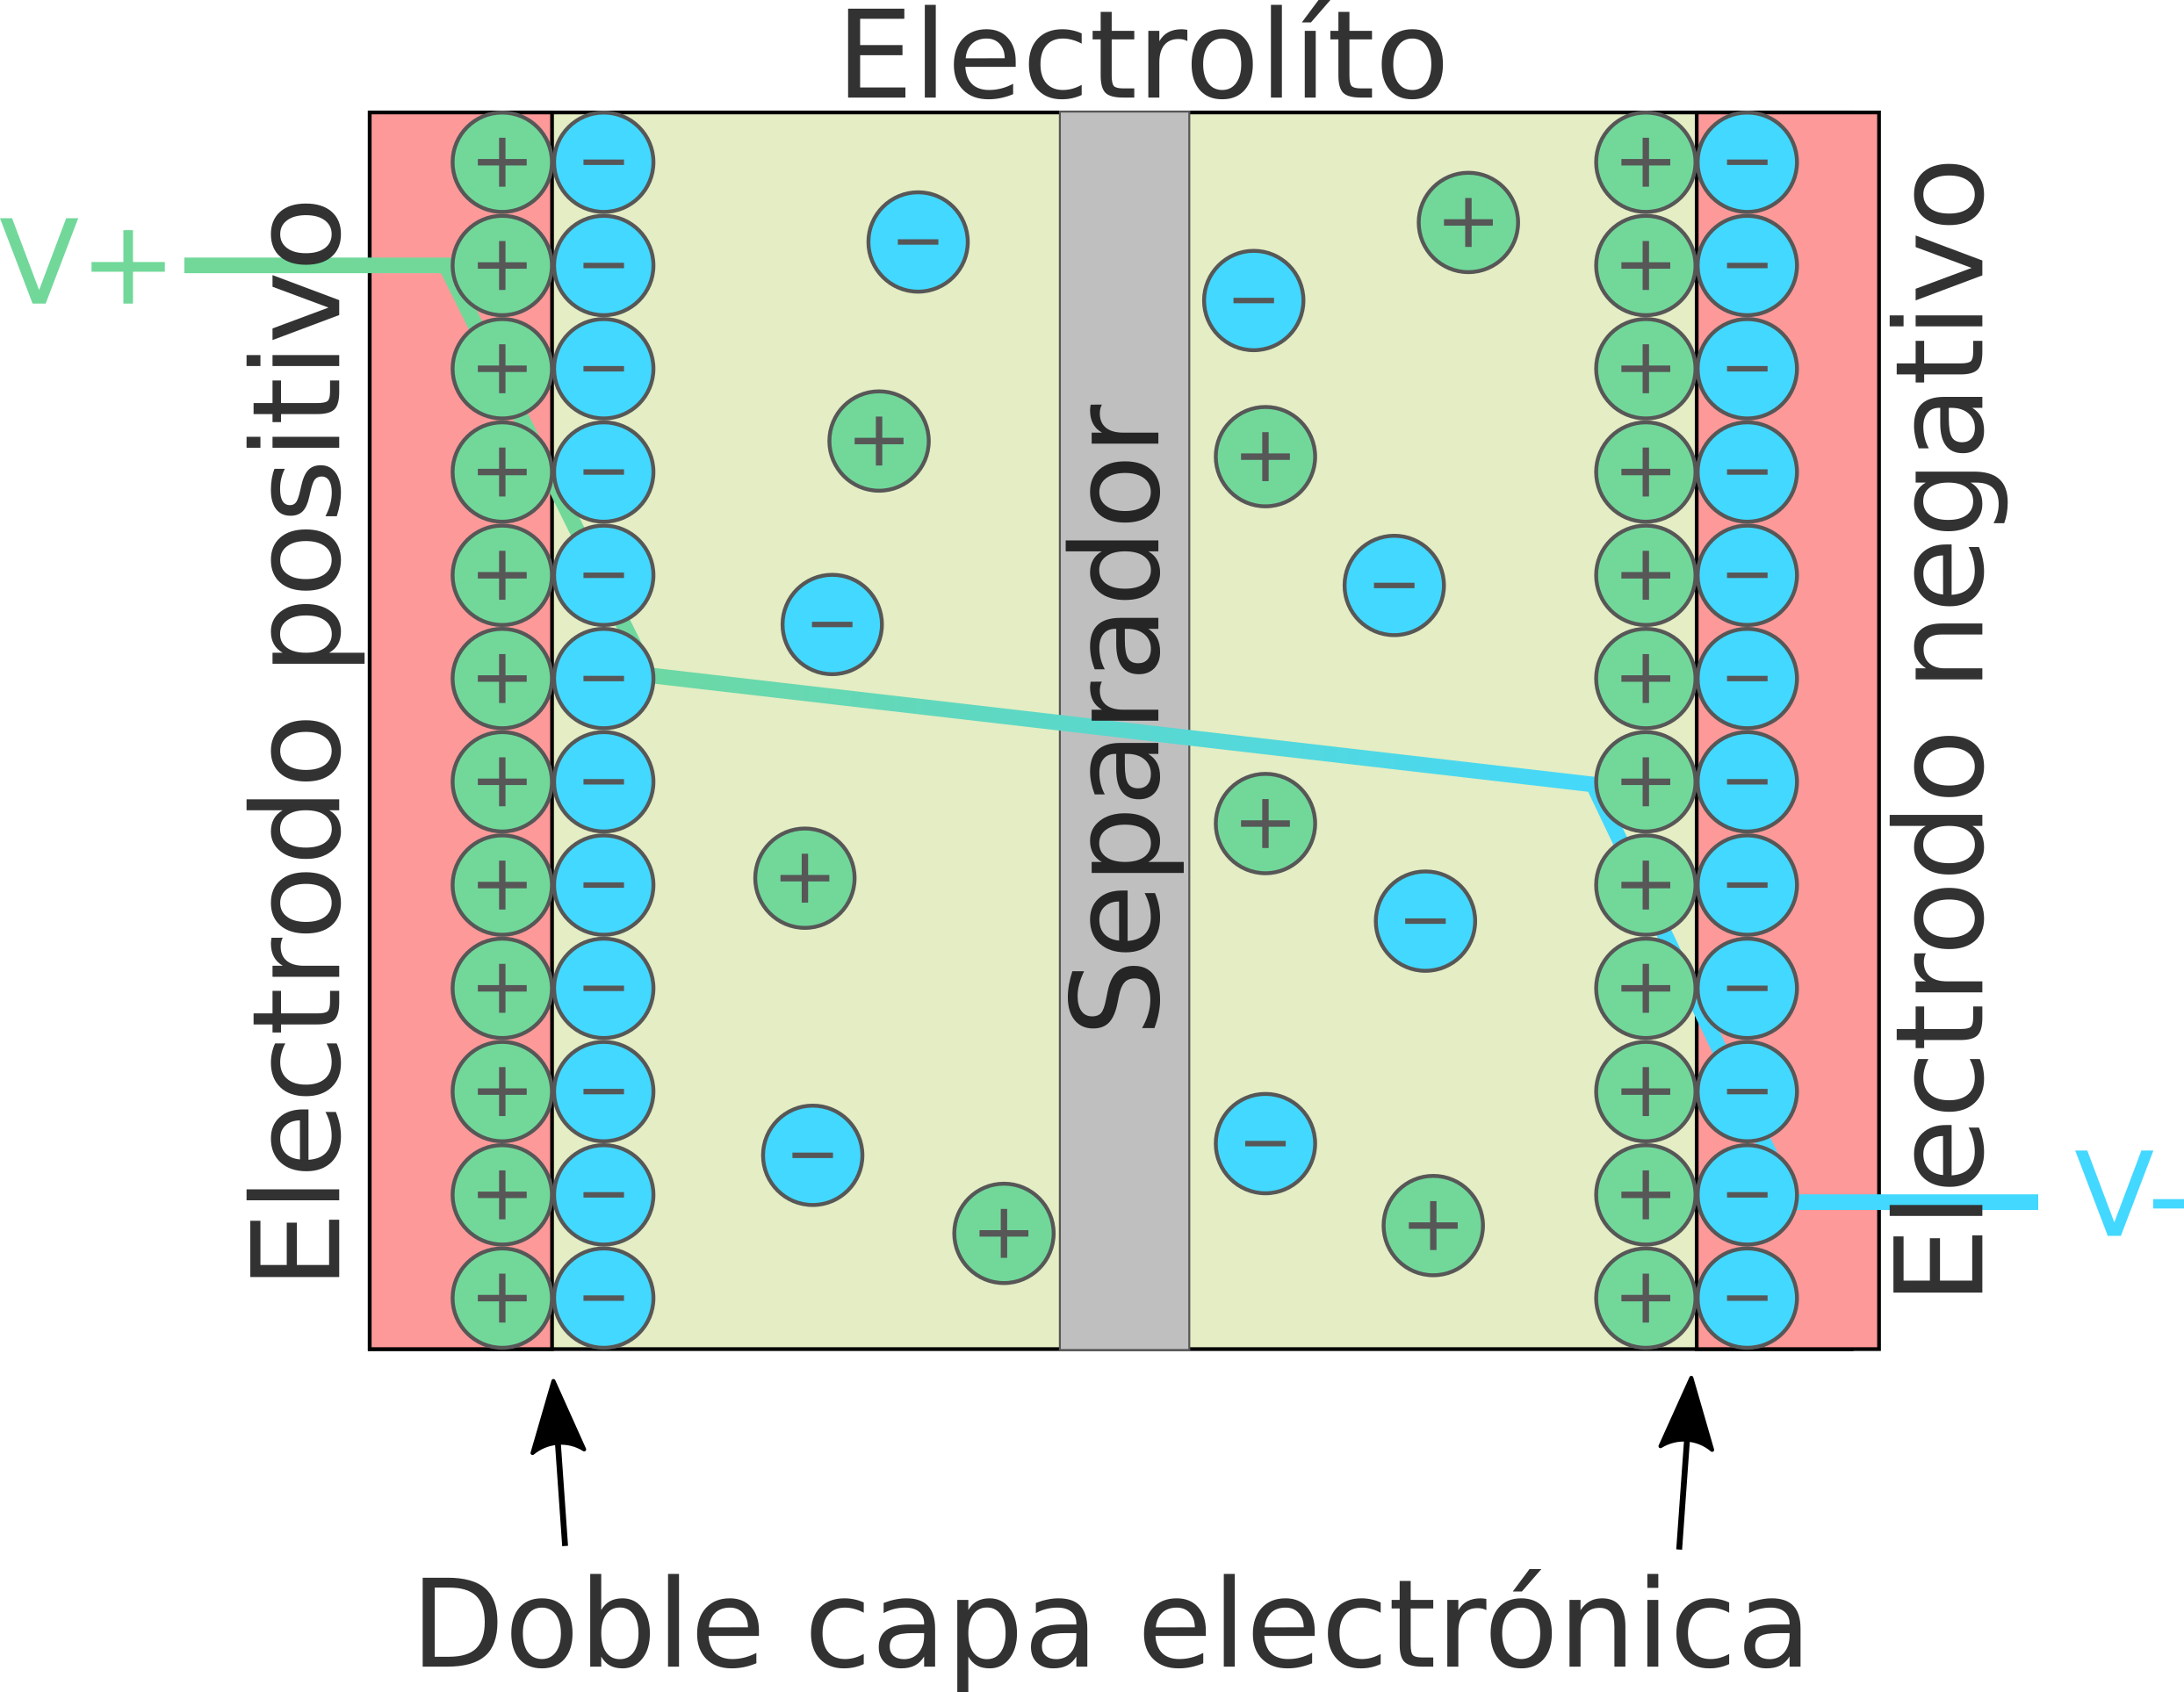
\includegraphics[width=0.7\textwidth]{edlc_schem.png}
		}
	\caption{Esquema de un supercondensador mostrando una doble capa electrónica de Helmholtz en cada electrodo.}
	\label{fig:edlc}
\end{figure}
\subsection{Pseudocapacitancia}